\documentclass[a4paper,10pt]{article}
\usepackage[utf8]{inputenc}
\usepackage{graphicx}

\newcommand{\myEmail}{marcschmid@gmx.ch}
\newcommand{\myWeb}{github.com/MWSchmid/Rcount}


%opening
\title{Rcount: User Guide}
\author{Marc W. Schmid, {\myEmail}}
%\address{Plant Developmental Genetics, Institute for Plant Biology, University of Z\"urich}
%\email{schmid.m@access.uzh.ch}

\begin{document}

\maketitle

\thispagestyle{empty}
\clearpage
\pagestyle{plain}
\pagenumbering{Roman}
\setcounter{page}{1}
% \begin{abstract}\noindent 
% PLACEHOLDER
% \newline
% \newline
% PLACEHOLDER
% \end{abstract}
% \clearpage
\tableofcontents
\clearpage
%%%%%%%%%%%%%%%%%%%%%%%%%%%%%%%%%%%%%%%%%%%%%%%%%%%%%%%%%%%%%%%%%%%%%%%%%%
\pagestyle{plain}
\pagenumbering{arabic}
\setcounter{page}{1}
% \section{Introduction}
% \clearpage
%%%%%%%%%%%%%%%%%%%%%%%%%%%%%%%%%%%%%%%%%%%%%%%%%%%%%%%%%%%%%%%%%%%%%%%%%%
\section{Installation}
This section describes how to obtain and install Rcount. Source code, 64-bit binaries for Linux, Windows, and Mac, and R-Scripts can be downloaded on {\myWeb}. The programs can easily use more than 3 Gb of RAM and it is therefore strongly recommended to use a 64-bit system with at least 6 Gb of RAM (see Table \ref{procData} for examples concerning the memory usage).
\subsection{Using pre-compiled binaries}
If you have a 64 bit (Ubuntu-like) Linux, Windows (7) or MacOSX, use the pre-compiled binaries. The binaries were built on Kubuntu 12.04, Windows 7, and MacOS 10.9 (versions below 10.9 were not tested). If you encounter problems with the binaries, try building the programs from source (see section \ref{buildInstructions}) and send a report to {\myEmail}.
\subsubsection{Linux}
Download and unpack the archive \texttt{linux\_64bit.zip}. Start Rcount-multireads, Rcount-format, and Rcount-distribute directly either by double-clicking on them or from the terminal (you may need to make them executable first, right-click on the binaries, open the ``properties'' dialog and check the box for ``is executable'' - or in a terminal type \texttt{chmod 755 filename}).
\subsubsection{Windows}
Download and unpack the archive \texttt{windows\_64bit.zip}. Start the applications directly by double-clicking on them.
\subsubsection{Mac}
Download and unpack the archive \texttt{mac\_64bit.zip}. Mount the \texttt{*.dmg} files (double-click) and start the applications by double-clicking on them.
\clearpage
%%%%%%%%%%%%%%%%%%%%%%%%%%%%%%%%%%%%%%%%%%%%%%%%%%%%%%%%%%%%%%%%%%%%%%%%%%
\section{Step-by-step example}
This section provides a step-by-step tutorial on how to get count tables starting from initial read files. The example data are from \textit{O. sativa} and comprises two ``sperm cell'' samples \cite{2013_Anderson}. Download and unpack the archive \texttt{rice\_tutorial.zip} from {\myWeb}. It contains a folder with the rice reference genome and its annotation in gff format (MSU7 from rice.plantbiology.msu.edu). It additionally contains pre-processed \texttt{.bam} and \texttt{.bai} files in case you would like to try only Rcount and to skip the download and alignment part of the tutorial (in this case go to section \ref{usePrePro}). The short reads download and alignment part is written for an Ubuntu-like Linux.
\subsection{OPTIONAL: Installation of additional programs}
Additional programs are required to download and align the short reads. It is later assumed that these programs reside in a folder that is included in your PATH environment variable. This can be done by either moving the programs into one of the by-default included folders (e.g. /usr/local/bin), or by adding the folder containing the programs to the PATH environment variable. Note that the latter is a temporary solution (the commands have to be entered each time you start a new terminal). Code for both options is given for each of the programs (note that the hash-tag \texttt{\#} stands for comments, which do not have to be typed into the terminal).
\begin{itemize}
 \item SRA toolkit\newline
Visit \texttt{www.ncbi.nlm.nih.gov/Traces/sra/sra.cgi?view=software}, download the archive for ``Ubuntu Linux 64 bit architecture'', unpack it, open a terminal, and type (adjust the path and version number):
\begin{verbatim}
# SOLUTION 1
cd /path/to/sratoolkit.x.x.x-x-ubuntu64/bin
sudo cp -r * /usr/local/bin
# SOLUTION 2 (temporary!)
export PATH="$PATH:/path/to/sratoolkit.x.x.x-x-ubuntu64/bin"
\end{verbatim}
 \item Bowtie2 \cite{2012_Langmead} \newline
Visit \texttt{bowtie-bio.sourceforge.net/bowtie2/index.shtml} and obtain the latest version. Follow the link in the box on the right side of the page, download the archive for linux, unpack it, open a terminal, and type (adjust the path and version number):
\begin{verbatim}
# SOLUTION 1
cd /path/to/bowtie2-x.x.x
sudo cp bowtie2* /usr/local/bin
# SOLUTION 2 (temporary!)
export PATH="$PATH:/path/to/bowtie2-x.x.x"
\end{verbatim}
\item TopHat2 \cite{2013_Kim} \newline
Visit \texttt{ccb.jhu.edu/software/tophat/index.shtml}, follow the link in the box on the right side of the page, download the latest version for linux (``Linux x86\_64 binary''), unpack it, open a terminal, and type (adjust the path and version number):
\begin{verbatim}
# SOLUTION 1
cd /path/to/tophat-2.x.x.Linux_x86_64
rm README
rm AUTHORS
rm COPYING
sudo cp * /usr/local/bin
# SOLUTION 2 (temporary!)
export PATH="$PATH:/path/to/tophat-2.x.x.Linux_x86_64"
\end{verbatim}
\item SAMtools \cite{2009_Li} \newline
Visit \texttt{sourceforge.net/projects/samtools/files/samtools/} and obtain the latest version. Download the archive and unpack it. SAMtools needs to be built from source. For this, install zlib (\texttt{zlib1g}, \texttt{zlib1g-dev}, and \texttt{zlib1g-dev} from the package manager), open a terminal, and type (adjust the path and version number):
\begin{verbatim}
# COMPULSORY - BUILD INSTRUCTIONS
cd /path/to/samtools-x.x.x
make
# SOLUTION 1
cd /path/to/samtools-x.x.x
sudo cp samtools /usr/local/bin
# SOLUTION 2 (temporary!)
export PATH="$PATH:/path/to/samtools-x.x.x"
\end{verbatim}
\end{itemize}
\subsection{OPTIONAL: Obtaining the short read data}
The data used in this tutorial can be conveniently retrieved from NCBI using the SRA toolkit. Open a terminal to download the example data (takes quite some time) in the working directory (e.g. rice\_tutorial, which has been automatically created by unpacking the archive \texttt{rice\_tutorial.zip}):
\begin{verbatim}
cd /path/to/rice_tutorial
fastq-dump SRR976339
fastq-dump SRR976340
\end{verbatim}
\subsection{OPTIONAL: Aligning the short reads to the reference genome}
The alignment of the short reads to the reference genome using TopHat2 requires an index of the reference genome. Build this index with (takes quite some time):
\begin{verbatim}
cd /path/to/rice_tutorial
bowtie2-build -f -q -o 0 all.chrs.con rice_genome_index
\end{verbatim}
You can now align the reads with TopHat2. Note that the option \texttt{-p 6} tells the computer to use six cores. You may need to change this according to your system. The options \texttt{-g 10} and \texttt{--no-coverage-search} are given to save memory and run-time (\texttt{-g 10} sets 10 as maximal number of alignments per read and \texttt{--no-coverage-search} omits searching novel exon-junctions using read coverage).
\begin{verbatim}
cd /path/to/rice_tutorial
mkdir SRR976339
mkdir SRR976340
tophat -p 6 -g 10 --no-coverage-search -o SRR976339 rice_genome_index SRR976339.fastq
tophat -p 6 -g 10 --no-coverage-search -o SRR976340 rice_genome_index SRR976340.fastq
\end{verbatim}
The Rcount-multireads program requires the \texttt{.bam} files to have an index (\texttt{.bai} file). Build this index with (takes few time):
\begin{verbatim}
cd /path/to/rice_tutorial/SRR976339
samtools index accepted_hits.bam
cd /path/to/rice_tutorial/SRR976340
samtools index accepted_hits.bam
\end{verbatim}
\subsection{Weighting reads that have more than one alignment with \textit{Rcount-multireads}}\label{usePrePro}
With the TopHat2 option \texttt{-g 10} enabled, it is possible that a read aligns to up to 10 locations in the genome. To avoid counting the read 10 times, we can weight these individual hits with Rcount-multireads. Start the program by clicking on it, specify the input file (\texttt{accepted\_hits.bam}) and a corresponding output file (e.g. \texttt{accepted\_hits\_weighted.bam}). Leave the allocation distance at 100 bp (approximately one read length). Press \texttt{OK} to start the weighting. This will take some minutes. Once the program has finished you can either process another file or close the program. Run the program on both samples (SRR976339 and SRR976340).
\subsection{Reformating the genome annotation with \textit{Rcount-format}}
The genome annotation has to be in a specific \texttt{.xml} format. You can create this file using Rcount-format. Start the program by clicking on it. Specify the input genome annotation file (\texttt{all.gff}, stored in your working directory), leave the rest unchanged, and press \texttt{Next} (this can take up to a minute or longer on older systems). You can now inspect the structure of the genome annotation. Click on ``gene'' to expand the menu. If you expand the entry ``mRNA'', you see five sub-entries (CDS, exon, five\_prime\_UTR, splice, and three\_prime\_UTR). Note that only exon and splice are important, considering that the other three types (CDS, five\_prime\_UTR, splice, and three\_prime\_UTR) are already included in the exons. Remove those three by changing their priority to 0 (double-click on the ``1'' to edit it) and click \texttt{Next}. Specify an output file (e.g. \texttt{Rcount\_rice\_annotation.xml} in your working directory) and click \texttt{Next}. Finally, close the program by clicking on \texttt{Finish}.
\subsection{Counting the number of hits per gene with \textit{Rcount-distribute}}
Use Rcount-distribute to count the number of reads per gene. Open the program and click \texttt{new} to create a new project. This will open a multi-tabbed dialog. For each sample, specify following files under the ``Files'' tab:
\begin{itemize}
\item Input {\textgreater} Annotation: \texttt{Rcount\_rice\_annotation.xml} \newline (stored in \texttt{/path/to/rice\_tutorial})
\item Input {\textgreater} Alignments: \texttt{accepted\_hits\_weighted.bam} \newline (stored in \texttt{/path/to/rice\_tutorial/SRR976339})
\item Output {\textgreater} Alignments: \texttt{accepted\_hits\_weighted\_mapped.bam} \newline (to be stored in \texttt{/path/to/rice\_tutorial/SRR976339})
\item Output {\textgreater} Counts: \texttt{SRR976339\_counts.txt} \newline (to be stored in \texttt{/path/to/rice\_tutorial})
\end{itemize}
Note that the example refers to the sample SRR976339. The \texttt{.bam} files can be found and should be stored in the corresponding folder (\texttt{/path/to/rice\_tutorial/SRR976339}). The count table should be stored in the working directory (\texttt{/path/to/rice\_tutorial}). Go to the ``Parameters'' tab and enable ``Use multiple alignments''. Leave the rest unchanged and click \texttt{OK}. A dialog will open and ask you to save the project (save it as \texttt{SRR976339.xml} in \texttt{/path/to/rice\_tutorial}). Once you have created for each sample a project, start the analysis by clicking \texttt{run all}. Once a sample is processed, the alignment statistics are automatically added to its project (saving is done automatically as well). 
\subsection{Merging the count tables in R}\label{R-usage}
Rcount-distribute creates for each sample a separate count table stored in the working directory (e.g. \texttt{SRR976339\_counts.txt}). The provided R-Script offers a function to read in all count tables from a given directory and merge them into a single table. Open R and use the following code to obtain a merged table and to generate a plot that gives a first impression of the data correlation and expression value distribution (table \ref{countTab} and figure \ref{allFigure}).
\begin{verbatim}
# set the path of the R-script provided
# see in linux_64bit.zip or windows_64bit.zip or mac_64bit.zip
pathToScript <- "/path/to/Rcount-R-functions.R"

# set the path to the folder where the count tables are located
pathToWorkingDirectory <- "/path/to/rice_tutorial"

# load the functions from the script
source(pathToScript)

# read in the count tables
# note that the expression values are rounded to integer numbers
# required by the downstream analysis programs
counts <- f.read.Rcount(pathToWorkingDirectory)

# save a merged table
outfile <- file.path(pathToWorkingDirectory, "all_counts.csv")
write.csv(counts, outfile)

# draw pairwise scatter-plots (unsorted/sorted) and histograms
f.pair.all(log2(counts+1), pathToWorkingDirectory)
\end{verbatim}
%
\begin{table}[!h]
\centering
\caption{The count table produced in the step-by-step example (type \texttt{head(counts)} in R to see this). }\label{countTab}
\vspace{8pt}
\begin{tabular}{l r r}
\hline
&SRR976339\_counts&SRR976340\_counts\\
\hline
LOC\_Os01g01019&13&10\\
LOC\_Os01g01030&55&35\\
LOC\_Os01g01040&127&111\\
LOC\_Os01g01060&70&47\\
LOC\_Os01g01080&5&10\\
LOC\_Os01g01115&28&10\\
\hline
\end{tabular}
\end{table}
%
\begin{figure}[!ht]
\begin{center}
\centering
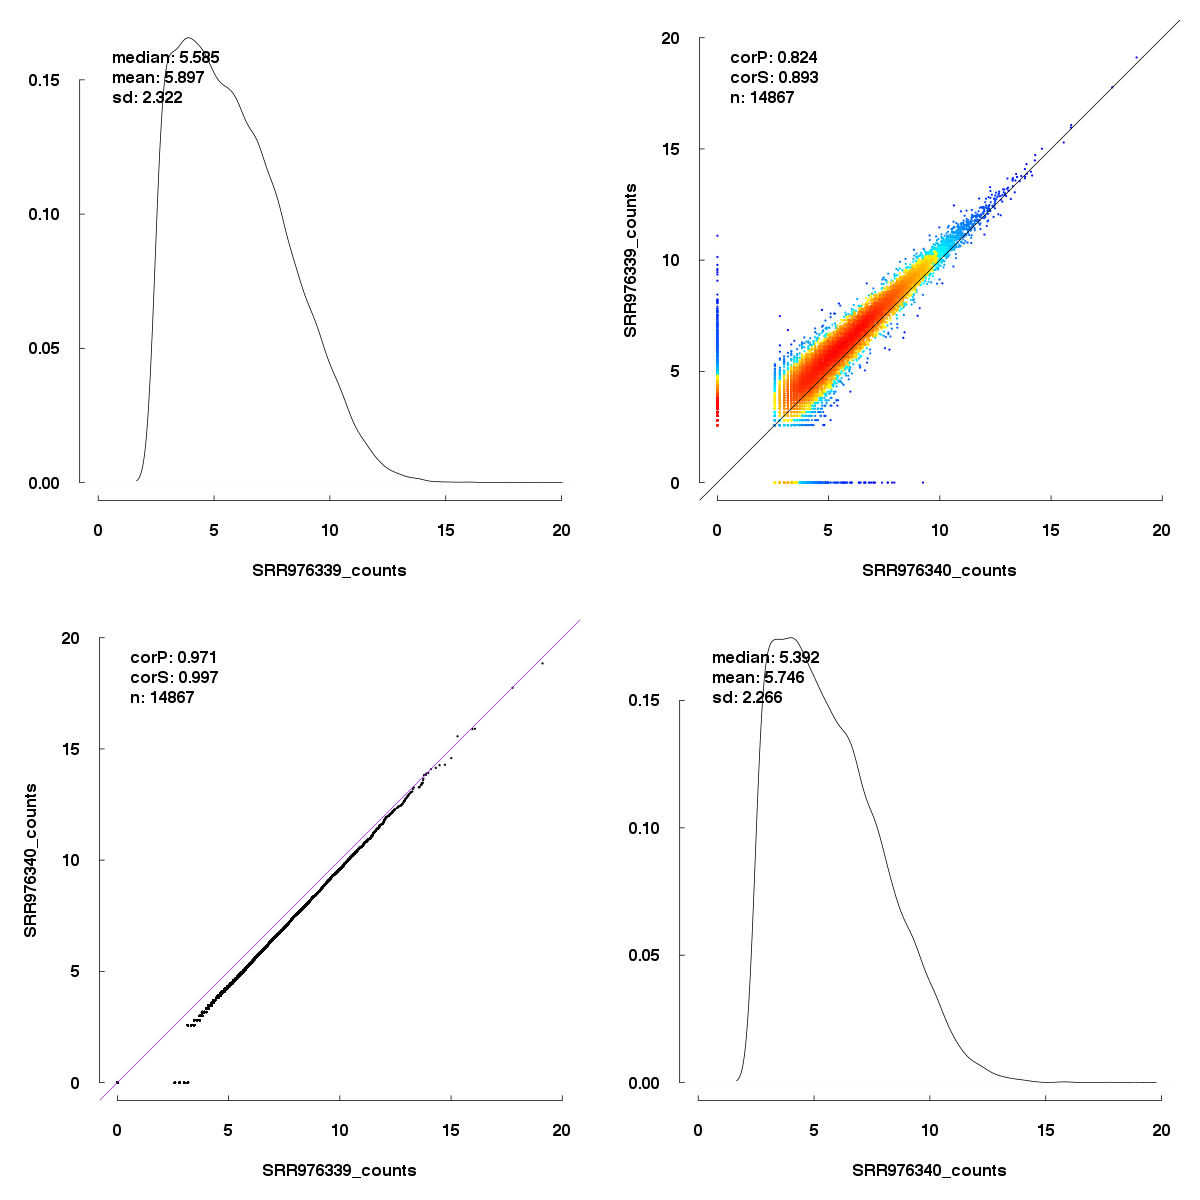
\includegraphics[width=5in]{userGuideFigure.png}
% 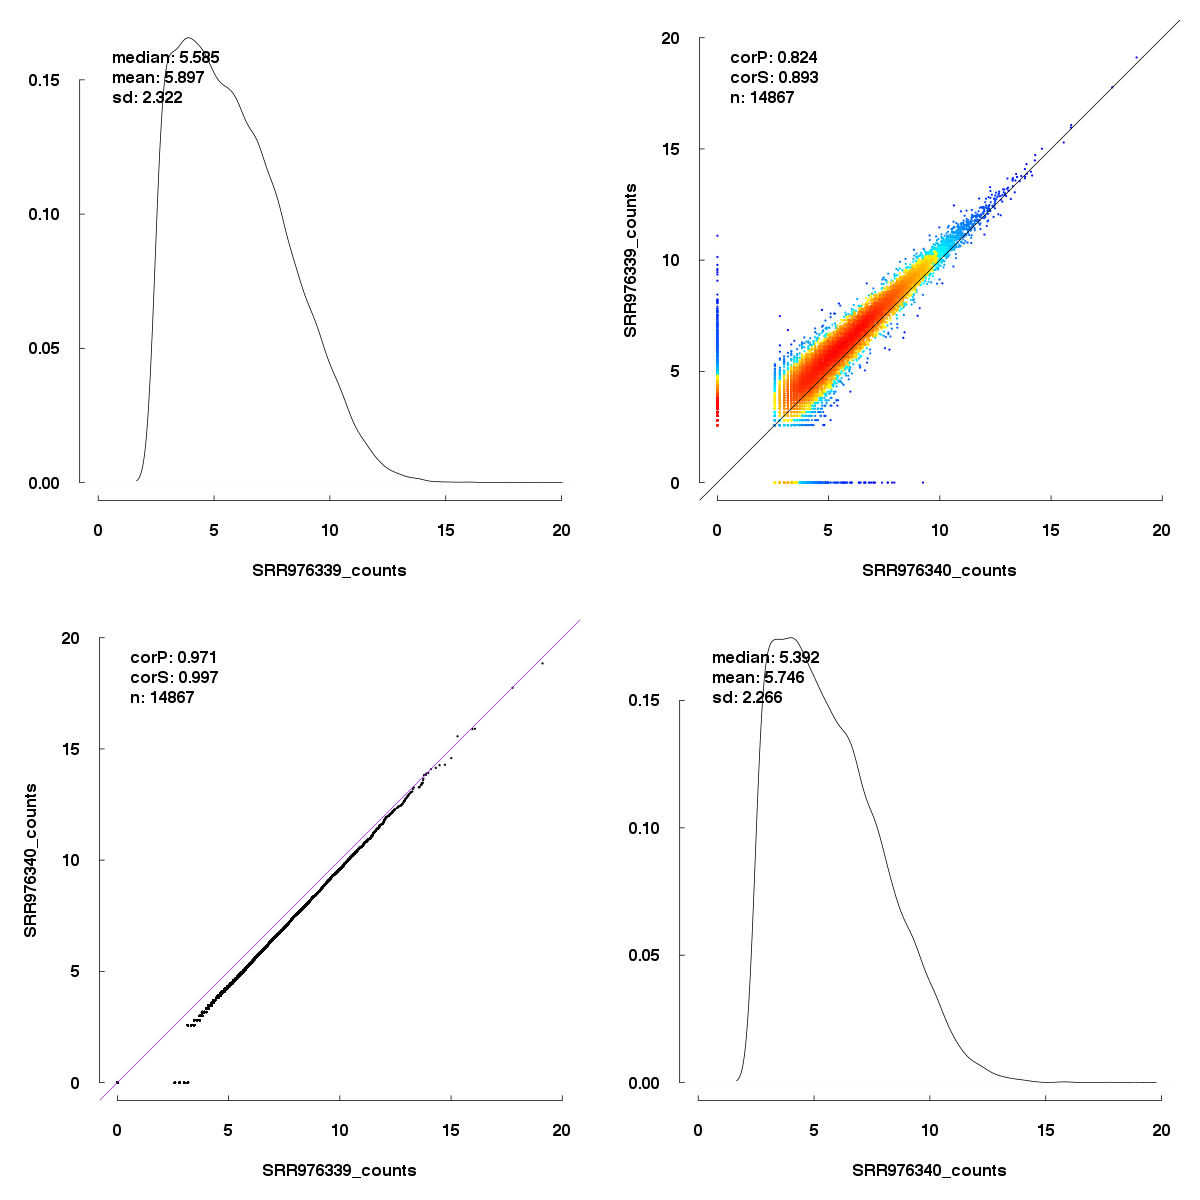
\includegraphics{userGuideFigure.png}
\end{center}
\caption{Distribution and pair-wise comparison of gene expression of the two samples processed in the step-by-step tutorial. The plots were generated with the function f.pair.all (included in the R-script). Top-left and bottom-right panels show the distributions of expression values for each sample. The panel on the top-right compares the gene expression values of the two samples (i.e. one dot reflects a gene). Colors indicate the point density: red and blue indicate the highest, respectively lowest, densities. The panel on the lower-left compares the sorted expression values of the two samples (i.e. one dot reflects the x-th highest expression value within one sample). The latter gives an indication of how similar the two distributions of expression values are (e.g. if a certain value means the same in both samples). Expression values correspond to log2(counts+1). CorP: Pearson correlation, CorS: Spearman correlation, n: number of genes plotted.}
\label{allFigure}
\end{figure}
\clearpage
%%%%%%%%%%%%%%%%%%%%%%%%%%%%%%%%%%%%%%%%%%%%%%%%%%%%%%%%%%%%%%%%%%%%%%%%%%%%%%%%%%%%%%%%%%%%%%%%%%%%%%%%%%%%%%%%%%%%%%%%%%%%%%%%%%%%%%%%%%%%%%%%%%%%%%%%%%%%%%%%%%%%%%%%%%%%%%%%%%%%%%%%%%%%%%%%%%%%%%%%%%%%%%%%%%%%%%%%%%%%%%
\section{Usage}
This section describes the features, requirements and parameters of Rcount in more detail. 
\subsection{Aligning the short reads}
After initial quality checks have been performed (e.g. with the FastQC software), the reads are aligned to a reference genome, preferentially with a splice-aware aligner. In the step-by-step example, we used TopHat2 \cite{2013_Kim} to align the reads. Other working examples are Subread \cite{2013_Liao} and STAR \cite{2013_Dobin}. In principle, any aligner works with Rcount, but some may require the \texttt{.bam} file to be additionally processed before using it. The following features of the \texttt{.bam} file are crucial for Rcount. 
\begin{itemize}
 \item \textit{The file must be sorted and an index must be present.}\newline
Rcount-multireads needs both, sorting and indexing. Rcount-distribute does not need an index, but sorting is strongly recommended (Rcount-multireads keeps the order intact, resorting is therefore not necessary).
 \item \textit{The \texttt{NH:i:x} tag must be present.}\newline
Without this tag, multireads are not recognized by Rcount-multireads and treated as unique alignments.
 \item \textit{There should not be any \texttt{XW} or \texttt{XM} tag. }\newline
Rcount uses \texttt{XW:f:x} to store the weights of reads with multiple alignments and \texttt{XM:i:x} for mapping statistics. The latter is similar to the \texttt{FLAG} column of a \texttt{.bam} file. The individual bits are explained in table \ref{bitTable}.
 \item \textit{The \texttt{CIGAR} string should only contain the operations \texttt{M, N, I, D, S, H}.}\newline
Other operations are not recognized by Rcount-distribute.
\end{itemize}
Note regarding paired-end reads: Rcount-distribute automatically takes the first read of one pair and ignores the second. 
\begin{table}[!h]
\centering
\caption{Description of the individual bits in the \texttt{XM:i:x} tag introduced by Rcount-distribute. }\label{bitTable}
\vspace{8pt}
\begin{tabular}{r l}
\hline
bit&description of the alignment\\
\hline
0x1&	belongs to a multiread \\
0x2&	has been skipped by Rcount-distribute \\
0x4&	contains gaps \\
0x8&	has a weight of zero \\
0x10&	maps to a known locus \\
0x20&	maps to a known exon \\
0x40&	maps to a known splice-junction \\
0x80&	maps to ambiguously several loci \\
\hline
\end{tabular}
\end{table}
\clearpage
%%%%%%%%%%%%%%%%%%%%%%%%%%%%%%%%%%%%%%%%%%%%%%%%%%%%%%%%%%%%%%%%%%%%%%%%%%%%%%%%%%%%%%%%%%%%%%%%%%%%%%%%%%%%%%%%%%%%%%%%%%%%%%%%%%%%%%%%%%%%%%%%%%%%%%%%%%%%%%%%%%%%%%%%%%%%%%%%%%%%%%%%%%%%%%%%%%%%%%%%%%%%%%%%%%%%%%%%%%%%%%
\subsection{\textit{Rcount-format}: Creating the genome annotation file}\label{annoDescription}
To overcome the large variety of genome annotation formats and their sometimes loose definition, Rcount uses a novel format which follows clear structural rules while still offering flexibility to add new features. The conversion of the most common formats (\texttt{.gtf, .gff, .bed}) into the \texttt{.xml} format is done by Rcount-format. Aside the format conversion, it also enables the user to edit some aspects of the genome annotation.
\begin{itemize}
 \item \textit{Loci and their transcripts can be extended on both sides.}\newline
Some samples have an abnormal number of hits in non-genic regions, often caused by hits directly flanking the known loci. Cases like this can be easily detected by comparing the results with and without the extension of the loci.
 \item \textit{Certain feature types can be removed by setting their priority to zero.}\newline
The genome annotation sometimes contains ambiguous information. For example, it often contains ``coding-sequence'' and ``UTR'' information. However, these are an \textit{in silico} specification of the type ``exon'' (i.e. exon already includes UTR and CDS), which behave identically during library preparation. Thus, they can be savely removed.
 \item \textit{Features can be given different priorities during the distribution of ambiguous reads.}\newline
Depending on the library preparation protocol, it is possible that some of the features in the genome annotation are very unlikely to be sequenced (e.g. rRNA-coding genes with poly(A)-selective library preparation protocols). Instead of removing these features entirely, it is possible to set a lower priority to them. In case a read aligns to a location where two features with different priorities overlap, it is automatically assigned to the one with a higher priority. It is important to note that priorities are only considered on a given level: In case of a gene and a pseudogene (top-level in the genome annotation structure), their priorities are only compared between each other. The pseudogene would not be compared to the gene's sub-feature ``mRNA''. Likewise, an ``mRNA'' is not compared to an ``exon''.
 \item \textit{Features must have three levels.}\newline
Rcount-distribute assumes three annotational levels, for example gene-mRNA-exon. Features without three levels are ignored.
 \item \textit{Specific requirements for BED files.}\newline
BED files must have at least 12 columns. An optional 13th column holds gene IDs (e.g. AT1G01010). It is assumed that the transcript ID is given as ``name'' in the fourth column (e.g. AT1G01010.1). The exons are constructed using the fields ``blockSizes'' and ``blockStarts'' (column 11 and 12). If there is no 13th column, the gene ID is per default inferred from the transcript ID by removing any \texttt{.X} at the end of the transcript ID (e.g. AT1G01010 in case of AT1G01010.1). The feature types are set per default to ``gene'', ``mRNA'', and ``exon''. Non-coding RNAs are identified by identical entries in the fields ``thickStart'' and ``thickEnd'' (column 7 and 8) and marked as ``non-coding-gene/RNA''. Rcount-format further assumes that the coordinates in the BED file are zero-based. 
 \item \textit{Verify that the annotation fits to the reference genome.}\newline
Fetching the annotation files (BED/GFF/GTF) from an online genome browser can be very convenient. However, it is important to ensure that the reads were aligned to a reference genome for which the annotation file was created (e.g. that the first chromosome is called ``Chr1'' in the fasta file as well as in the BED/GFF/GTF file). It is therefore recommended to download both, the reference sequence and the genome annotation from the same resource.
\end{itemize}
For convenience, several pre-processed genome annotations (\textit{A. thaliana}, \textit{B. taurus}, \textit{C. elegans}, \textit{C. familiaris}, \textit{D. melanogaster}, \textit{G. gallus}, \textit{H. sapiens}, \textit{M. musculus}, and \textit{R. norvegicus}) are provided on {\myWeb} in the archive \texttt{test\_data\_annotations.zip}. They were build with the data available on tophat.cbcb.umd.edu/igenomes.shtml using the ``ENSEMBL data source''. The archives on this website also contain pre-built bowtie and bwa indices, which can directly be used in conjunction with the provided genome annotation. To create the individual \texttt{.xml} genome annotations, the \texttt{genes.gtf} files were first pre-processed with the python script (\texttt{convertCufflinksGTFforRcount.py}) supplied in the archives \texttt{linux\_64bit.zip}, \texttt{windows\_64bit.zip}, and \texttt{mac\_64bit.zip} and then processed using Rcount-format (with the ENSEMBL option enabled). Each of the genome annotation has been tested with a random sample from SRA (see section \ref{testDataPart} for more details).
%%%%%%%%%%%%%%%%%%%%%%%%%%%%%%%%%%%%%%%%%%%%%%%%%%%%%%%%%%%%%%%%%%%%%%%%%%%%%%%%%%%%%%%%%%%%%%%%%%%%%%%%%%%%%%%%%%%%%%%%%%%%%%%%%%%%%%%%%%%%%%%%%%%%%%%%%%%%%%%%%%%%%%%%%%%%%%%%%%%%%%%%%%%%%%%%%%%%%%%%%%%%%%%%%%%%%%%%%%%%%%
\subsection{\textit{Rcount-multireads}: Weighting reads with more than one alignment}
Some organisms have very large gene families with similar sequence. To avoid underestimation of expression values of transcripts with similar sequence, one can allow multiple alignments of one read to several locations in the genome. However, a read $r$ with $m > 1$ alignments would count $m$ times, resulting in overestimation of expression values. To overcome this, Rcount-multireads calculates for each alignment $i$ of such a read the weight $H_{i}$ using a ``score'' $S_{i}$ divided by the sum of scores from all alignments of the read ($H_{i} = S_{i} / \sum_{i = 1}^{m} S_{i}$). If $\sum_{i = 1}^{m} S_{i}$ is zero, all alignments of the respective read are discarded (i.e. all weights set to zero). For ungapped alignments, the score is defined as sum of coverage originating from uniquely aligned reads at the position of the alignment and the surrounding region. The size of the region can be set by choosing the ``allocation distance''. This value will be added on both sides of the alignment position. For gapped alignments, the score equals to the number of uniquely aligned reads spanning the same gap. Thus, if a read has both types of alignments, the ungapped ones are generally preferred.
\newline
\newline
Further notes:
\begin{itemize}
 \item \textit{Rcount-multireads is not required for Rcount-distribute to run.} \newline
If you do not use reads with multiple alignments, you can safely skip Rcount-multireads. It is important that the number of unique alignments is well above the number of multireads. If not, it is better to use only the uniquely aligned reads (high number of multireads was observed especially in amplified libraries where the cDNA was prepared using random primers, [in-house data]).
 \item \textit{Memory usage is mainly influenced by the number of multireads.} \newline
The main memory consumption of Rcount-multireads is caused by storing the multireads. The size of the reference genome does not make a big difference. If RAM is limiting, one could lower the maximum number of alignments per read. 
 \item \textit{Known issues on Mac and Windows.} \newline
The progress bar is not updated instantly. It instead advances directly to 80 \% after finishing reading the files.
 \item \textit{Rcount-multireads may be substituted by any other program that adds weights to reads with multiple alignments.} \newline
Rcount-multireads adds the tag \texttt{XW:f:x} to specify the weights of reads with multiple alignments. The sole requirement for alternative algorithms is the possibility to add the weights in the form of the \texttt{XW:f:x} tag. An example for an alternative software may be CSEM \cite{2011_Chung} (available on deweylab.biostat.wisc.edu/csem), which was originally developed for ChIP-Seq data analysis using multireads. It calculates the posterior probabilities for all alignments of a multiread and stores them the \texttt{ZW:f:x} tag. This tag can be renamed using the following code (example given for an ubuntu-like linux). However, it is important to note that CSEM does not handle gapped alignments in a specific way (treats them as regular alignment). Also, we experienced that summing up the posterior probabilities results in a slightly higher number than the number of reads with multiple alignments (thus, one tends to slightly overweight the multireads).
\begin{verbatim}
# an example of CSEM usage (instead of Rcount-multireads)
# download, unpack, and compile CSEM (deweylab.biostat.wisc.edu/csem) 
cd /path/to/csem
make

# add CSEM to your PATH (temporary!)
export PATH="$PATH:/path/to/csem"

# alignments need to be sorted by read names for CSEM
# however, they are sorted by position in the step-by-step tutorial
# to resort the alignments you need samtools
cd /path/to/rice_tutorial/SRR976339
samtools sort -n accepted_hits.bam byName

# run CSEM to add the posterior probabilities (ZW:f:x tag)
run-csem --bam --no-extending-reads byName.bam 100 withPP

# rename/copy the ZW tag into XW
# (the backslash indicates that all should be written on one single line)
samtools view -h withPP.sorted.bam |\
sed 's/ZW:f:/XW:f:/g' |\
samtools view -bS - > withPP_retagged.bam

# you can now use withPP_retagged.bam directly within Rcount-distribute
\end{verbatim}
% samtools view -h csem_output.sorted.bam | \
% sed 's/ZW:f:/XW:f:/g' | \
% samtools view -bS - > csem_output.replaced.sorted.bam
% This tag can be copied and renamed using the python script (\texttt{reformatCSEMbam.py}) supplied in the archives \texttt{linux\_64bit.zip}, \texttt{windows\_64bit.zip}, and \texttt{mac\_64bit.zip}. However, it is important to note that CSEM does not handle gapped alignments in a specific way (treats them as regular alignment).
\end{itemize}
\clearpage
%%%%%%%%%%%%%%%%%%%%%%%%%%%%%%%%%%%%%%%%%%%%%%%%%%%%%%%%%%%%%%%%%%%%%%%%%%%%%%%%%%%%%%%%%%%%%%%%%%%%%%%%%%%%%%%%%%%%%%%%%%%%%%%%%%%%%%%%%%%%%%%%%%%%%%%%%%%%%%%%%%%%%%%%%%%%%%%%%%%%%%%%%%%%%%%%%%%%%%%%%%%%%%%%%%%%%%%%%%%%%%
\subsection{\textit{Rcount-distribute}: Mapping aligned reads to genomic features}
To count the number of reads per genomic feature, the positions of the aligned reads (termed ``hits'') have to be mapped to the genomic features. Hits are matched to the genomic features as follows: ungapped hits must be entirely within one exon of a given gene and gapped hits must accurately span exon junctions (corresponds to the intersection\_strict mode in HTSeq). Hits can be divided into unambiguous (mapping to transcripts of only one locus) and ambiguous (mapping to transcripts of more than one locus). To avoid counting ambiguous hits multiple times, Rcount-distribute proportionally distributes them based on the number of unambiguous hits. If there are no unambiguous hits, the ambiguous hits are equally distributed. However, we assume a case where two loci A and B overlap such that locus A is entirely located within locus B. Locus A shall be ``truly'' expressed (i.e. is \textit{in vivo} expressed and therefore has reads mapping to it), locus B not (i.e all reads that map to B are coming from A). Using a single step, all hits of locus A would be declared as ambiguous. In case locus B has no unambiguous hit, the hits from locus A would be equally distributed to locus A and B, leading to an underestimation of the expression value from locus A and an overestimation of the expression value from locus B (a false positive). In another case where locus B has one or two unambiguous hits due to sequencing and/or alignment errors, all the hits from locus A would be wrongly assigned to locus B (one false positive and one false negative). The same error would occur if locus A has a longer transcript \textit{in vivo} than the \textit{in silico} genome annotation would indicate. The hits at the borders of locus A would then be unambiguously assigned to locus B and as a consequence also all the ambiguous hits. To overcome this scenario at least to some extent Rcount-distribute uses a two step approach. In the first step, all hits are mapped to all annotated transcripts. In many cases one can expect that each ``truly'' expressed transcript should have at least some hits within the first few bps at its 3' end because the library preparation protocols frequently rely on poly(A)-tail priming for cDNA synthesis. In addition, one can set a minimal number of hits. Transcripts not matching these criteria are then discarded. During the second step, the hits are then divided into unambiguous and ambiguous. The unambiguous hits are assigned first and used to distribute the ambiguous hits. The transcripts are then filtered again using the same criteria as before. The final expression value of a locus is then calculated as the sum of hits assigned to any of its transcripts.
\newline
\newline
Rcount-distribute takes a genome file (\texttt{.xml}) and an alignment file (\texttt{.bam}) as input. As a result, it writes a new \texttt{.bam} file with the mapping tag \texttt{XM:i:x} and a count table. All parameters are set while creating a new project and stored in the project file. Additionally, one can enable the use of strand information if (!) the library preparation protocol was strand specific (note that Rcount checks for strand equality). This greatly helps to assign the ambiguous reads as overlapping genes are often in opposite orientation to each other. Note that in case of paired-end reads, only the first/forward read is used.
% \newline
% \newline
%Note regarding alignment statistics: If the sample has an enormous number of hits (75 million still worked), the number given in the statistics may be wrong (due to maximal size of floating point numbers). However, the count tables are not affected by this and still correct.
%\clearpage
%%%%%%%%%%%%%%%%%%%%%%%%%%%%%%%%%%%%%%%%%%%%%%%%%%%%%%%%%%%%%%%%%%%%%%%%%%%%%%%%%%%%%%%%%%%%%%%%%%%%%%%%%%%%%%%%%%%%%%%%%%%%%%%%%%%%%%%%%%%%%%%%%%%%%%%%%%%%%%%%%%%%%%%%%%%%%%%%%%%%%%%%%%%%%%%%%%%%%%%%%%%%%%%%%%%%%%%%%%%%%%
\subsection{Reading and merging tables in R}
Rcount-distribute creates for each sample a separate count table with multiple columns:
\begin{itemize}
 \item \texttt{sumUnAmb}: number of unambiguously mapped hits.
 \item \texttt{sumAmb}: number of ambiguously mapped hits before distributing them accoring to the number of unambiguously mapped hits.
 \item \texttt{sumAllo}: number of ambiguously mapped hits after distributing them accoring to the number of unambiguously mapped hits.
 \item \texttt{sumDistUnAmb, sumDistAmb, sumDistAllo} are identical to \texttt{sumUnAmb, sumAmb, sumAllo}, but only within the first x bp from the 3' of the transcript. The value x can be specified in Rcount-distribute by enabling ``consider 3' bias''.
 \item \texttt{TH}: total number of hits (equals to \texttt{sumUnAmb+sumAllo}).
\end{itemize}
The provided R-Script offers a function to read in all table files from a given directory and merge them into a single table (see section \ref{R-usage}). The function \texttt{f.read.Rcount} loads per default the column ``TH''. Other columns in the count tables can be loaded using the argument \texttt{toReturn} of the function \texttt{f.read.Rcount} (e.g. \texttt{f.read.Rcount(pathToWorkingDirectory, toReturn = 'sumUnAmb')}). 
\clearpage
%%%%%%%%%%%%%%%%%%%%%%%%%%%%%%%%%%%%%%%%%%%%%%%%%%%%%%%%%%%%%%%%%%%%%%%%%%%%%%%%%%%%%%%%%%%%%%%%%%%%%%%%%%%%%%%%%%%%%%%%%%%%%%%%%%%%%%%%%%%%%%%%%%%%%%%%%%%%%%%%%%%%%%%%%%%%%%%%%%%%%%%%%%%%%%%%%%%%%%%%%%%%%%%%%%%%%%%%%%%%%%
\section{Test data}\label{testDataPart}
Rcount was tested with data from multiple organisms with different genome sizes and RNA-Seq libraries (table \ref{testData}). Genome annotation data and genome indices were obtained as described before (see section \ref{annoDescription}) from tophat.cbcb.umd.edu/igenomes.shtml. Short reads were downloaded from www.ncbi.nlm.nih.gov/sra. The reformatted \texttt{.xml} genome annotation, as well as the resulting project files and count tables, can by found on {\myWeb} in the archives \texttt{test\_data\_annotations.zip} and \texttt{test\_data\_results.zip}. Reads were aligned with TopHat2 (version 2.0.11 \cite{2013_Kim}) allowing up to 10 alignments per read (-g 10). For increasing the speed of TopHat2, the coverage-search was turned off for all data. Allocation distance for weighting multireads was set to 50 for all samples. Run-time and memory usage were obtained on a 64 bit Kubuntu (12.04) running on an Intel{\textregistered} {Core$^{\textup{TM}}$} i7 930@2.8 GHz with 24 Gb RAM. Input and output files were read and written from the same hard-drive (Samsung HD, 7'200 rpm). Memory usage of Rcount-multireads is mostly influenced by the number of reads with multiple alignments (e.g. high memory requirements for the mouse sample compared to the human sample). However, for Rcount-distribute, the size of the genome annotation has the largest impact on the memory usage (e.g. the xml file holding the genome annotation of the human genome is with 643 Mb almost double the size compared to the xml genome annotation file for the mouse genome, table \ref{procData}).
%%%%%%%%%%%%%%%%%%%%%%%%%%%%%%%%%%%%%%%%%%%%%%%%%%%%%%%%%%%%%%%%%%%%%%%%%%
\begin{table}[!h]
\centering
\caption{Data used to test Rcount.}\label{testData}
\vspace{8pt}
\begin{tabular}{l l l r}
\hline
organism&assembly&accession&\# reads\\
\hline
% \textit{A. thaliana}	&TAIR10		&SRR847501\cite{2013_Loraine}		&26'956'447	\\
\textit{A. thaliana}	&TAIR10		&SRX275909\cite{2013_Loraine}		&52'181'949	\\
\textit{B. taurus}	&Btau4.0	&DRR001892\cite{2013_Takeo}		&69'040'753	\\
\textit{C. elegans}	&WS220		&SRR1015366\cite{2014_Washburn}		&34'542'067	\\
\textit{C. familiaris}	&BROADD2	&DRR001151		&113'253'542	\\
\textit{D. melanogaster}&BDGP5.25	&SRR629969\cite{2013_Ramaswami}		&31'267'571	\\
\textit{G. gallus}	&WASHUC2	&SRR1264638\cite{2014_Ku}		&20'189'799	\\
\textit{H. sapiens}	&GRCh37		&DRR000897\cite{2011_Odawara}		&22'635'328	\\
\textit{M. musculus}	&NCBIM37	&DRR013118\cite{2014_Yukawa}		&27'028'925	\\
\textit{R. norvegicus}	&RGSC3.4	&SRR1041766\cite{2014_Cortez}		&28'897'182	\\
\hline
\end{tabular}
\end{table}
%%%%%%%%%%%%%%%%%%%%%%%%%%%%%%%%%%%%%%%%%%%%%%%%%%%%%%%%%%%%%%%%%%%%%%%%%%
\begin{table}[!h]
\centering
\caption{Alignment statistics, approximate run-time and memory usage of Rcount using the test data given in Table \ref{testData}. Note that the number of multireads only includes the ones with at least one alignment with a weight above zero.}\label{procData}
\vspace{8pt}
\begin{tabular}{l r r r r r r}
\hline
organism&\multicolumn{2}{r}{\# reads aligned}&\multicolumn{2}{r}{Rcount-multireads}&\multicolumn{2}{r}{Rcount-distribute}\\
&unique&multiple&time&memory&time&memory\\
\hline
\textit{A. thaliana}	&41'098'964	&2'231'636	&12 min	&1.0 Gb	&18 min	&1 Gb	\\
\textit{B. taurus}	&34'913'558	&3'538'481	&15 min	&1.1 Gb	&18 min	&928 Mb	\\
\textit{C. elegans}	&25'492'284	&1'889'021	&10 min	&729 Mb	&14 min	&1.0 Gb	\\
\textit{C. familiaris}	&66'816'362	&4'809'058	&18 min	&2.8 Gb	&22 min	&878 Mb	\\
\textit{D. melanogaster}&25'806'514	&969'484	&9 min	&216 Mb	&12 min	&981 Mb	\\
\textit{G. gallus}	&10'465'361	&158'067	&2 min	&185 Mb	&4 min	&803 Mb	\\
\textit{H. sapiens}	&16'056'845	&2'169'498	&5 min	&1.0 Gb	&13 min	&3.3 Gb	\\
\textit{M. musculus}	&9'630'768	&7'898'165	&8 min	&3.2 Gb	&8 min	&1.7 Gb	\\
\textit{R. norvegicus}	&21'729'100	&1'288'736	&10 min	&410 Mb	&12 min	&1.2 Gb	\\
\hline
\end{tabular}
\end{table}
\clearpage
%%%%%%%%%%%%%%%%%%%%%%%%%%%%%%%%%%%%%%%%%%%%%%%%%%%%%%%%%%%%%%%%%%%%%%%%%%%%%%%%%%%%%%%%%%%%%%%%%%%%%%%%%%%%%%%%%%%%%%%%%%%%%%%%%%%%%%%%%%%%%%%%%%%%%%%%%%%%%%%%%%%%%%%%%%%%%%%%%%%%%%%%%%%%%%%%%%%%%%%%%%%%%%%%%%%%%%%%%%%%%%
\section{Building from source}\label{buildInstructions}
If the binaries are not working or you would like to implement a new feature, you can build them from the source code. 
\subsection{Linux}
Compiling the programs using QtCreator is quite easy.
\begin{itemize}
\item download and unpack the archive \texttt{source.zip}
\item install QtCreator (on the Ubuntu repository: \texttt{qtcreator}) - make sure to use Qt 4.x.x libraries.
\item install zlib (on the Ubuntu repository: \texttt{zlib1g}, \texttt{zlib1g-dev}, \texttt{zlib1g-dev}), which is required by Rcount-multireads and Rcount-distribute
\item start QtCreator and open each of the *.pro files
\begin{itemize}
\item Rcount-format: \texttt{../source/p502\_format\_wizard/p502\_format\_wizard.pro}
\item Rcount-multireads: \texttt{../source/p502\_process\_multireads/p502\_process\_multireads.pro}
\item Rcount-distribute: \texttt{../source/p502dataAnalysisRNA/p502dataAnalysisRNA.pro}
\end{itemize}
\item for Rcount-multireads and Rcount-distribute, copy the seqan folder into one of your general include paths (e.g. \texttt{sudo cp -r seqan /usr/local/include}) or add a line \texttt{INCLUDEPATH += <path containing seqan folder>} into the *.pro files. For Rcount-format, seqan is not required and this step can therefore be skipped.
\item finally, in the QtCreater menu select \texttt{Build > Build Project ``my\_project''}
\end{itemize}
\subsection{Windows}
Compiling on Windows requires access to VisualStudio. The following steps worked well with VisualStudio 2010 Ultimate.
\begin{itemize}
\item download and unpack the archive \texttt{source.zip}
\item install the Qt Add-In for VisualStudio - make sure to use Qt 4.x.x libraries.
\item open each of the *.pro files (\texttt{Qt > Open Qt Project File (.pro)...})
\begin{itemize}
\item Rcount-format: \texttt{../source/p502\_format\_wizard/p502\_format\_wizard.pro}
\item Rcount-multireads: \texttt{../source/p502\_process\_multireads/p502\_process\_multireads.pro}
\item Rcount-distribute: \texttt{../source/p502dataAnalysisRNA/p502dataAnalysisRNA.pro}
\end{itemize}
\item for Rcount-format, compile the code with \texttt{Build > Build Solution}
\item for Rcount-multireads and Rcount-distribute
\begin{itemize}
\item download the latest zlib from zlib.net (e.g. \texttt{zlib-1.2.8.tar.gz}) and unpack the archive
\item open the project properties (right-click on the project in the solution explorer) and do the following steps:
\begin{itemize}
\item under \texttt{Configuration Properties > VC++ Directories}, in the field \texttt{Include Directories}, add the zlib folder
\item under \texttt{Configuration Properties > VC++ Directories}, in the field \texttt{Include Directories}, add the folder containing the seqan folder
\item under \texttt{Configuration Properties > General}, change the variable \texttt{Character Set} to \texttt{Use Multi-Byte Character Set}
\item under \texttt{Configuration Properties > C/C++ > Preprocessor} in the field \texttt{Preprocessor Definitions}, remove the \texttt{UNICODE} key-words and add the key-word \texttt{\_CRT\_SECURE\_NO\_WARNINGS}
\item under \texttt{Configuration Properties > C/C++ > Command Line}, add the options \texttt{-W2 -wd4996} in the field with the \texttt{Additional Options}
\end{itemize}
\item close the project properties and compile it with \texttt{Build > Build Solution}
\end{itemize}
\end{itemize}
\subsection{Mac}
Currently, there are no build instructions available for the MacOS.
% due to Qt 5 instead of 4: #include <QtWidgets> wherever one has #include <QtGui>; in the pro file QT += ... widgets; in main.cpp #include <QtGui/QApplication> becomes to #include <QtWidgets/QApplication> 
% also due to Qt: QChar ...toAscii() replaced by toLatin1()
% in the .pro file INCLUDEPATH+= ../zlib-1.2.8 \ ../ and LIBS += -lZ
% in main.cpp before QApplication a(...), add the lines:
%     QString path = QString(argv[0]);
%     QString end = path.split("/").last();
%     path.remove(path.length() - end.length(), end.length());
%     QDir dir(path);
%     dir.cdUp();
%     dir.cd("PlugIns");
%     QApplication::setLibraryPaths(QStringList(dir.absolutePath()));
% then: /Users/stefan/Applications/Qt/5.3/clang_64/bin/macdeployqt xy.app -always-overwrite -dmg
%
\clearpage
%%%%%%%%%%%%%%%%%%%%%%%%%%%%%%%%%%%%%%%%%%%%%%%%%%%%%%%%%%%%%%%%%%%%%%%%%%%%%%%%%%%%%%%%%%%%%%%%%%%%%%%%%%%%%%%%%%%%%%%%%%%%%%%%%%%%%%%%%%%%%%%%%%%%%%%%%%%%%%%%%%%%%%%%%%%%%%%%%%%%%%%%%%%%%%%%%%%%%%%%%%%%%%%%%%%%%%%%%%%%%%
\bibliography{userGuideReferences}
%\bibliographystyle{elsart-harv}
\bibliographystyle{elsart-num}

\end{document}
